%Basics
\documentclass[aps, prl, reprint, a4paper, english, 12pt]{revtex4}
\usepackage[utf8]{inputenc}
\usepackage{babel}

%Symbols and scientifics
\usepackage{amsmath}
\usepackage{commath}
\usepackage{amsfonts}
\usepackage{amssymb}
\usepackage{physics}
\usepackage{mathtools}
\usepackage{siunitx}
\sisetup{
per-mode = fraction ,
round-mode = figures ,
round-precision = 3 ,
scientific-notation = engineering ,
output-decimal-marker = {.} ,
exponent-product = \times ,
separate-uncertainty = true ,
uncertainty-separator = \ ,
output-product = \cdot ,
quotient-mode = fraction ,
range-phrase = - ,
range-units =  single ,
inter-unit-product = \ensuremath{{\cdot{}}} ,
number-unit-product = \ ,
multi-part-units = single ,
}
\usepackage{units}

%Appendix, TOC and Bibliography
\usepackage{appendix}
\renewcommand\appendixtocname{Appendices}
%\usepackage[nottoc]{tocbibind}
\usepackage[lastpage,user]{zref}

%Figures
\usepackage[svgnames]{xcolor} % Required to specify font color
\usepackage{tikz}
\usetikzlibrary{shadings}
\usepackage{float}
\usepackage{rotating}
\usepackage{graphicx}
\usepackage{caption}
\usepackage{wrapfig}
\usepackage[rmargin=2.5cm, tmargin=2.5cm, lmargin=2.5cm, bmargin=2.5cm]{geometry}
\usepackage{xcolor}
\usepackage{etoolbox}
\usepackage{verbatim}
\usepackage[space]{grffile}
\usepackage[final]{pdfpages}
\usepackage{array}
\usepackage{multirow}

%Header footer
\usepackage{fancyhdr}
\pagestyle{fancy}
\lhead{F. G. Kristensen,\\C. V. Sørensen og R. K. F. Wiuff}
\chead{Phonon mechanics in graphene membranes\\}
\rhead{28/9-2017\\Course 34029: Physics Project}
\cfoot{Side \thepage\, af \zpageref{LastPage}}
\renewcommand{\headrulewidth}{0.4pt}
\renewcommand{\footrulewidth}{0.4pt}

%Text tools
\usepackage[normalem]{ulem}
\usepackage{import}
\usepackage{newclude}
\usepackage{url}
\usepackage{lipsum}
\usepackage{microtype}
\usepackage{hyperref}
\hypersetup{
  colorlinks   = true, %Colours links instead of ugly boxes
  urlcolor     = blue, %Colour for external hyperlinks
  linkcolor    = blue, %Colour of internal links
  citecolor   = red %Colour of citations
}
\usepackage[capitalise]{cleveref}
\usepackage{enumitem}
\usepackage{booktabs}
\usepackage{natbib}
\usepackage{silence}
\WarningFilter{revtex4-1}{Repair the float}

%Definitions and new commands
\setlength{\parindent}{0pt}
\setlength{\parskip}{1ex plus 0.5ex minus 0.2ex}
\newcommand{\logas}[1]{\log_{_{10}}{\left( #1 \right)}}
\newcommand{\sins}[1]{\sin{\left( #1 \right)}}
\newcommand{\tans}[1]{\tan{\left( #1 \right)}}
\newcommand{\coss}[1]{\cos{\left( #1 \right)}}
\newcommand{\sinas}[1]{\sin{\left( #1 \degr \right)}}
\newcommand{\tanas}[1]{\tan{\left( #1 \degr\right)}}
\newcommand{\cosas}[1]{\cos{\left( #1 \degr\right)}}
\newcommand{\lnas}[1]{\mathrm{ln}\left( #1 \right)}
\newcommand{\degr}{^{\circ}}
\newcommand{\me}{\mathrm{e}}
\newcommand{\eula}[1]{ \dpd{L }{#1} - \dod{}{t}\left(\dpd{L}{\dot{#1}}\right)}


\begin{document}

%Titlepage herunder:
\begin{abstract}
  \begin{description}
    \item[Background] My money's in that office, right? If she start giving me some bullshit about it ain't there, and we got to go someplace else and get it, I'm gonna shoot you in the head then and there.
    \item[Purpose] My money's in that office, right? If she start giving me some bullshit about it ain't there, and we got to go someplace else and get it, I'm gonna shoot you in the head then and there.
    \item[Method] My money's in that office, right? If she start giving me some bullshit about it ain't there, and we got to go someplace else and get it, I'm gonna shoot you in the head then and there.
    \item[Results] My money's in that office, right? If she start giving me some bullshit about it ain't there, and we got to go someplace else and get it, I'm gonna shoot you in the head then and there.
    \item[Conclusion] My money's in that office, right? If she start giving me some bullshit about it ain't there, and we got to go someplace else and get it, I'm gonna shoot you in the head then and there.
  \end{description}
\end{abstract}

\title{Nanomechanics for graphene membranes}
\date{10/1-2018}
\author{Frederik Grunnet Kristensen (s164003)}
\email[E-mail at ]{s164003@student.dtu.dk}
\author{Christoffer Vendelbo Sørensen (s163965)}
\email[E-mail at ]{s163965@student.dtu.dk}
\author{Rasmus Kronborg Finnemann Wiuff (s163977)}
\email[E-mail at ]{s163977@student.dtu.dk}
\affiliation{Technical University of Denmark}
\homepage[Homepage of the Technical University of Denmark ]{dtu.dk}

\maketitle

\pagenumbering{arabic}

\tableofcontents
\thispagestyle{empty}
\newpage
\setcounter{page}{1}

%Text
\lipsum{60}
%Text

%Bibliography herunder:
\newpage

\bibliographystyle{unsrtnat}
\bibliography{Bibliography}

\newpage
\listoffigures
\listoftables
\newpage
%Appendicer herunder:
% !TEX root = Main.tex

\appendix
\appendixpage
\addappheadtotoc
%\section{Animation of \nth{9} mode}
%\begin{center}
%  \animategraphics[autoplay,loop,width=\textwidth]{60}{VNL/Frames/frame}{1}{60}
%\end{center}
%Section 1 herunder:
\section{NanoSheetCreator.py}
\label{NSCstart}
\inputminted[python3=true,bgcolor=Black,linenos=true]{python}{VNL/PythonScripts/NanoSheetCreator.py}
\label{NSCend}
%Section 2 herunder:
\todo[inline]{Correct graph}
\begin{figure}
  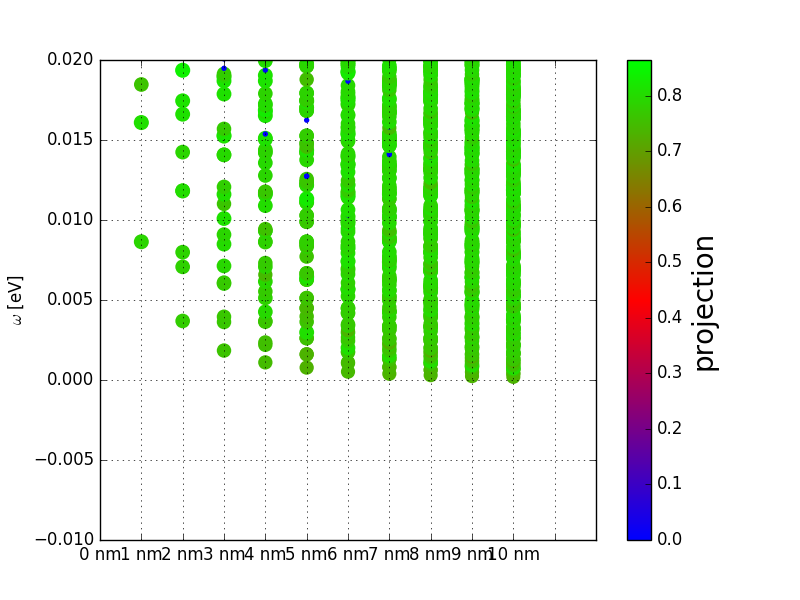
\includegraphics[width=\textwidth]{VNL/PythonScripts/FrequencyVSSize/PlottingArea/FrequencyModeProjections.eps}
  \caption{$\omega(r)$}
  \label{OR}
\end{figure}
\newpage

\end{document}
